%%%%%%%%%%%%%%%%%%%%%%%%%%%%%%%%%%%%%%%%%%%%%%%%%%%%%%%%%%%%%%%%%%%%%%%%%%%%%%%%%
% Beamer presentationtion 															
% LaTeX Template 																
% Version 1.0 (10/11/12)														%
% This template has been downloaded from: http://www.LaTeXTemplates.com 		%
% https://www.sharelatex.com/blog/2013/08/14/beamer-series-pt2.html
% https://www.writelatex.com/docs?snip_uri=http://www.latextemplates.com/templates/presentations/1/presentation_1.zip				
% License: CC BY-NC-SA 3.0 (http://creativecommons.org/licenses/by-nc-sa/3.0/)  
% Compilar: pdflatex ficheiroTex.tex
%%%%%%%%%%%%%%%%%%%%%%%%%%%%%%%%%%%%%%%%%%%%%%%%%%%%%%%%%%%%%%%%%%%%%%%%%%%%%%%%%

%----------------------------------------------------------------------------------------
%	PACKAGES AND THEMES
%----------------------------------------------------------------------------------------

\documentclass[10pt]{beamer}

\mode<presentation> {

% The Beamer class comes with a number of default slide themes
% which change the colors and layouts of slides. Below this is a list
% of all the themes, uncomment each in turn to see what they look like.

%\usetheme{default}
%\usetheme{AnnArbor}
%\usetheme{Antibes}
%\usetheme{Bergen}
%\usetheme{Berkeley}
%\usetheme{Berlin}
%\usetheme{Boadilla}
%\usetheme{CambridgeUS}
%\usetheme{Copenhagen}
%\usetheme{Darmstadt}
%\usetheme{Dresden}
%\usetheme{Frankfurt}
%\usetheme{Goettingen}
%\usetheme{Hannover} OK
%\usetheme{Ilmenau} OK
%\usetheme{JuanLesPins}
%\usetheme{Luebeck} OK
%\usetheme{Madrid}
%\usetheme{Malmoe}
%\usetheme{Marburg}
%\usetheme{Montpellier}
%\usetheme{PaloAlto}
%\usetheme{Pittsburgh}
%\usetheme{Rochester}
%\usetheme{Singapore}
%\usetheme{Szeged}
%\usetheme{Warsaw}
\usetheme[progressbar=frametitle]{metropolis}
% As well as themes, the Beamer class has a number of color themes
% for any slide theme. Uncomment each of these in turn to see how it
% changes the colors of your current slide theme.

%\usecolortheme{albatross}
%\usecolortheme{beaver}
%\usecolortheme{beetle}
%\usecolortheme{crane}
%\usecolortheme{dolphin}
%\usecolortheme{dove}
%\usecolortheme{fly}
%\usecolortheme{lily}
%\usecolortheme{orchid}
%\usecolortheme{rose}
%\usecolortheme{seagull}
%\usecolortheme{seahorse}
%\usecolortheme{whale}
%\usecolortheme{wolverine}

%\setbeamertemplate{footline} % To remove the footer line in all slides uncomment this line
%\setbeamertemplate{footline}[page number] % To replace the footer line in all slides with a simple slide count uncomment this line

%\setbeamertemplate{navigation symbols}{} % To remove the navigation symbols from the bottom of all slides uncomment this line
}
\usepackage{appendixnumberbeamer}
\usepackage{booktabs}
\usepackage[scale=2]{ccicons}
\usepackage{pgfplots}
\usepgfplotslibrary{dateplot}
\usepackage{xspace}
\newcommand{\themename}{\textbf{\textsc{metropolis}}\xspace}
%\usepackage{graphicx} % Allows including images
%\usepackage{booktabs} % Allows the use of \toprule, \midrule and \bottomrule in tables
%\usepackage[utf8]{inputenc} %Permite a utilização dos carateres portugueses
\usepackage{verbatim} %Permite inserir os comentários
%\usepackage{graphicx} %Permite inserir gráficos
%\usepackage[portuguese]{babel} % Para termos texto em português, e.g. legendas e datas
%\usepackage[english]{babel}
%\setbeamertemplate{caption}[numbered] %para numerar os captions
%\usepackage[labelfont=scriptsize,labelfont=bf,font=scriptsize,belowskip=-15pt,aboveskip=5pt]{caption}

%----------------------------------------------------------------------------------------
%	Otimização da gestão de instalações desportivas nas empresas municipais
%   Aplicação de uma abordagem baseada na gestão por processos
%----------------------------------------------------------------------------------------

\title[Dropout Prediction]{Dropout Prediction: A Systematic Literature Review} 
\subtitle{SLR Dropout} 
% The short title appears at the bottom of every slide, the full title is only on the title page

\begin{comment} % Estrutura da apresentação

\end{comment}

\author{Pedro Sobreiro, José Garcia Alonso, Javier Berrocal} % Your name
\institute[UNEX] % Your institution as it will appear on the bottom of every slide, may be shorthand to save space
{ 
University of Extremadura ~~~~~~~~~~~~~~~% Your institution for the title page
\medskip
\textit{pdealexa@alumnos.unex.es} % Your email address
}
\date{Webinar, 26 June 2020} % Date, can be changed to a custom date

\begin{document}

\begin{frame}
	\titlepage % Print the title page as the first slide
\end{frame}

\begin{frame}
\frametitle{Summary} % Table of contents slide, comment this block out to remove it
\tableofcontents % Throughout your presentation, if you choose to use \section{} and \subsection{} commands, these will automatically be printed on this slide as an overview of your presentation

\end{frame}

%----------------------------------------------------------------------------------------
%	PRESENTATION SLIDES
%----------------------------------------------------------------------------------------

%------------------------------------------------
\section{Research goals} % Sections can be created in order to organize your presentation into discrete blocks, all sections and subsections are automatically printed in the table of contents as an overview of the talk
%------------------------------------------------
\begin{comment}
Dropout predicting is challenging analysis process which requires appropriate approaches to address the dropout. Existing approaches are applied in different areas such as education, telecommunications, retail, social networks, and banking services. The goal is to identify customers in the risk of dropout to support retention strategies. This research developed a systematic literature review to evaluate the development of existing studies to predict dropout using machine learning,  following the guidelines recommended by Kitchenham and Peterson. The systematic review followed three phases planning, conducting and reporting. The selection of the most relevant articles was based on the use of Active Systematic Review tool using artificial intelligence algorithms. The criteria identified 28 articles and several research lines where identified. Dropout is a transversal problem for several sectors of economic activity, where it can be taken countermeasures before it happens if detected early.
\end{comment}

\begin{frame}
	\frametitle{Research goals}
	% Vamos colocar os objetivos do estudo 
	\Large{What is the current state of machine learning research studies to predict dropout in contractual settings?}

	
\end{frame}

\section{Introduction} % A subsection can be created just before a set of slides with a common theme to further break down your presentation into chunks
\begin{comment}
Esta investigação, desenvolvida através da técnica de inquérito por questionário, pretende avaliar como é que esses docentes encararam essa realidade. O trabalho de campo foi realizado na primeira quinzena de abril de 2020 envolvendo docentes de uma instituição de ensino superior portuguesa tendo-se obtido 35 respostas válidas.

\end{comment}

\begin{frame}
	\frametitle{Introduction}
	\Large
	\textbf{Data mining}\\
		\begin{itemize} \normalsize
			\item Customer analysis is fundamental to develop business and marketing intelligence \footnotesize(Sheth, Mittal, \& Newman, 1998)\normalsize, supporting the understanding of historical data identifying trends and patterns \footnotesize(Berry \& Linoff, 2004)\normalsize
			\item This process is also known as data mining, the extraction of knowledge from data (Han \& Kamber, 2006)

		\end{itemize}	

	
	
	\tiny
	~~~~Allen, I. E., \& Seaman, J. (2011). Going the Distance: Online Education in the United States, 2011. Em Sloan Consortium (NJ1). Obtido de https://eric.ed.gov/?id=ED529948 \\
	~~~~Martinho, D. S. (2014). O Ensino Online nas Instituições de Ensino Superior Privado. As perspetivas: Docente e discente e as implicações na tomada de decisão institucional.\\
	~~~~McCarthy, S. A. (2009). Online Learning as a Strategic Asset. Volume I: A Resource for Campus Leaders. A Report on the Online Education Benchmarking Study Conducted by the APLU-Sloan National Commission on Online Learning. Em Association of Public and Land-grant Universities. Obtido de https://eric.ed.gov/?id=ED517308\\

\end{frame}

\section{Methodology}
\begin{comment}
The data was anonymised, removing all personal information before being retrieved from the management system.
Esta investigação, desenvolvida através da técnica de inquérito por questionário, pretende avaliar como é que esses docentes encararam essa realidade. O trabalho de campo foi realizado na primeira quinzena de abril de 2020 envolvendo docentes de uma instituição de ensino superior portuguesa tendo-se obtido 35 respostas válidas.
\end{comment}
\begin{frame}
	\frametitle{Methodology}
	\begin{itemize}
		\item Was developed a Systematic Literature Review (SLR) developed in three stages \footnotesize(Kitchenham \& Charters, 2007)\normalsize: Plan, Conduct and Report;
		\item Plan: definition of the research need, identification of the research questions and the development of the review protocol;
		\item Conduct: research identification, study selections, quality assessment, data extraction, finishing with the data synthesis;
		\item Report: stage that develops the activity report review.
	\end{itemize}
	\tiny 
	~~~~Kitchenham, B., \& Charters, S. (2007). Guidelines for performing structural literature reviews in software engineering (pp. 1–26) [Joint technical report]. Australia: Keele Univ., and Empirical Software Eng., Nat’l ICT.\\

\end{frame}

\begin{frame}
	\frametitle{Systematic Literature Review Phases}
	\begin{figure}
		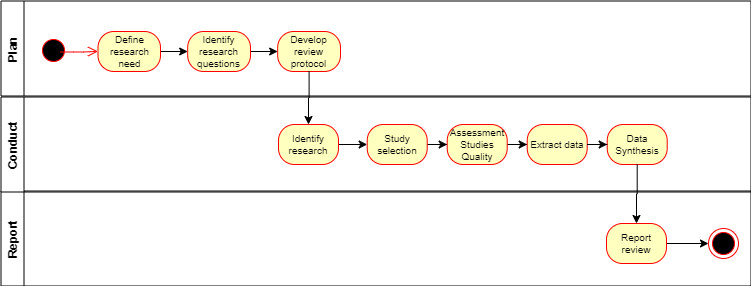
\includegraphics[scale=0.5]{../img/slr_phases.png}
		\caption{SLR phases based on Kitchenham and Charter (2007)}
		\label{figure1}
	\end{figure}
\end{frame}

\begin{frame}
	\frametitle{Research questions}
	What is the current state of machine learning research studies to predict dropout in contractual settings? Based in this question were identified the following questions:
	\begin{itemize}
		\item RQ1: What studies have been published?;
		\item RQ2: Which algorithms have been used to predict the dropout?
		\item RQ3: What are the more relevant features related to predicting customer dropout?
		\item RQ4: When the dropout occurs? 
		\item RQ5: What is the accuracy of the machine learning algorithms to predict dropout?
	\end{itemize}
\end{frame}
\begin{comment}
RQ1: aims to identify what researches have been published so far in the area. This will allow to understand the extent of the research being developed. 
RQ2: aim to identify which different types of machine learning algorithms used to predict the dropout (RQ2) to deep the knowledge of the approaches being used to address the dropout. 
RQ3: explores which features are being used to predict the dropout. 
RQ4: Intends to understand if the timing related to the customer dropout is considered, this question explores if any study explores the advantage of using survival analysis, considering that allows also to examine if an event occurs but also how long took to occur (Williams, 2008). This perspective entails the understanding if is also covered the timings of the dropout event in the potential research to be explored. 
RQ5: aims to identify the accuracy of machine learning algorithms to predict the dropout. The goal of the prediction in the dropout is to develop classification task,  according to Rätsch (2004) is to find a functional mapping between the input data X, describing the input pattern, to a class label Y, such that Y=f(X), where the aim is to accurately predict the correct label on unseen data. However should be used appropriate performance measures, e.g. if the data is imbalanced should be considered the use of accuracy (Chawla, Bowyer, Hall, & Kegelmeyer, 2002)
\end{comment}

\begin{frame}
	\frametitle{Population, Intervention, Comparison, Outcomes and Context}
\begin{center}
\begin{table}
  \centering
  \scriptsize
  \caption{
  	PICOC criteria
  	}
    \begin{tabular}{p{3cm} p{5cm}}
    \toprule
    PICOC & Description\\
    \midrule
	Population & Research papers about dropout with contractual settings \\ \hline
	Intervention &  Machine learning algorithms to predict dropout	\\ \hline	
	Comparison & Studies addressing machine learning algorithms to predict dropout \\ \hline 
	Outcome & Synthesis identifying research questions, gaps in the research domain and also best practices identified \\ \hline
	Context & Academia and industry\\
\bottomrule
\end{tabular}
\label{Abordagens analisadas}
\begin{flushleft}
	Note: Context (PICOC) as suggested Kitchenham and Charters (2007) and proposed by Petticrew and Roberts (Petticrew \& Roberts, 2006) to support the development of the search string.
\end{flushleft}
\end{table}
\end{center}
	\tiny 
~~~~Kitchenham, B., \& Charters, S. (2007). Guidelines for performing structural literature reviews in software engineering (pp. 1–26) [Joint technical report]. Australia: Keele Univ., and Empirical Software Eng., Nat l ICT.\\
~~~~Petticrew, M., \& Roberts, H. (2006). Systematic reviews in the social sciences: A practical guide. Malden, MA ; Oxford: Blackwell Pub.\\
\end{frame}

\begin{frame}
	\frametitle{Search }
	\begin{itemize}
		\item Search string: ((“customer dropout”) OR (“customer churn”) AND “machine learning” AND (“contractual” OR “membership”));
		\item Applied to the title, abstract, and keywords in the search period between January 2000 and June 2020
		\item The exclusion criteria were Books, Non-English articles, patents, and thesis
		\item The selection process was developed using ASReview (ASReview Core Development Team, 2019) creating a dataset of the identified articles, providing five relevant papers and five irrelevant papers to train Machine Learning model Naïve Bayes;
		\\~\\
	\end{itemize}
		\tiny 
~~~~Kitchenham, B., \& Charters, S. (2007). Guidelines for performing structural literature reviews in software engineering (pp. 1–26) [Joint technical report]. Australia: Keele Univ., and Empirical Software Eng., Nat l ICT.\\
~~~~Petticrew, M., \& Roberts, H. (2006). Systematic reviews in the social sciences: A practical guide. Malden, MA ; Oxford: Blackwell Pub.\\
\end{frame}


\section{Results}
\begin{comment} 

\end{comment}

\begin{frame}[fragile]{Results}
  	\begin{itemize}
		\item Os resultados revelam que a maioria dos professores que responderam ao questionário são do sexo masculino (56\%)
		\item Questionados sobre a avaliação da qualidade do ensino online versus ensino presencial 24\% considera que é inferior, 44\% refere que não existem diferenças e 26\% por vezes é superior
		\item Quando confrontados com gosto pelo ensino online em relação ao seu gosto pelo ensino presencial 6\% considera inferior, 29\% por vezes inferior, 21\% não apresenta preferência, 38\% acha que é por vezes superior e 6\% considera superior
		\item Em relação à disponibilidade para o ensino online em relação à sua disponibilidade para o ensino presencial 18\% apresenta mais disponibilidade para o ensino online, 41\% considera a sua disponibilidade por vezes superior, 35\% é indiferente e 6\% considera ter menos disponibilidade.
	\end{itemize}
\end{frame}

\begin{frame}[fragile]{Resultados}
  	\begin{itemize}
		\item Quando questionados sobre os aspetos tecnológicos, 100\% apresenta experiência de mais de 6 anos na utilização processadores de texto e email. 97\% PowerPoint e motores de busca;
		\item Em relação a ferramentas de videoconferência verifica-se que 56\% dos respondentes têm mais de 6 anos de experiência com o Zoom, 21\% de 3 a 6 anos e 24\% até 3 anos de experiência
		\item Na utilização de ferramentas para chat 76\% mais de 6 anos, 15\% de 3 a 6 anos, 6\% menos de 3 e 3\% não apresentava nenhuma experiência
		\item Na utilização do Moodle 53\% apresentava mais de 6 anos de experiência, 29\% 3 a 6 anos e 18\% menos de 3 anos
	\end{itemize}
\end{frame}

\begin{frame}[fragile]{Resultados}
  	\begin{itemize}
		\item A análise de correlação mostrou relações com elevado significado estatístico entre a qualidade do ensino online versus ensino presencial* e: (1) gosto em ensinar presencialmente (r\textsubscript{s}=.51,p$<$.01); (2) disponibilidade para o ensino online (r\textsubscript{s}=.44,p$<$.01); (3) preferência por testes online (r\textsubscript{s}=.46,p$<$.01); (4) preferência com apresentações orais(r\textsubscript{s}=.40,p$<$.05); (5) experiência com chat (r\textsubscript{s}=.36,p$<$.05);
		\item Não se identificaram relações significativas entre qualidade do ensino online e: (1) idade, (2) anos docência, (2) satisfação com Moodle, Zoom e Google Docs;
	\end{itemize}
	\tiny * Escala de likert com as opções: 1-Inferior; 2- Por vezes inferior; 3 – Sem diferenças significativas ; 4-Por vezes superior;  5-Superior 

\end{frame}


\section{Conclusion}
\begin{frame}
	\frametitle{Discussão e Conclusões}
	\begin{itemize}

 		\item A dimensão da amostra não permite a generalização dos resultados obtidos pelo que o trabalho de campo vai continuar com o alargamento da amostra dos respondentes para outras instituições do ensino superior;

		\item Pretende-se ainda investigar outros aspetos, nomeadamente como é que os professores perspetivam o ensino online para o desenvolvimento dos estudantes, da sua carreira profissional e das instituições de ensino superior;


	\end{itemize}
	\tiny 
\end{frame}


\begin{frame}
\frametitle{Obrigado!}
\normalsize
	Pedro Sobreiro - IPSantarém  \\~\\
	Domingos Martinho - ISLA Santarém \\~\\
	Marco Tereso - ISLA Santarém \\~\\
\end{frame}


\end{document}\grid
